% Foliensatz: "AFu-Kurs nach DJ4UF" von DK0TU, Amateurfunkgruppe der TU Berlin
% Lizenz: CC BY-NC-SA 3.0 de (http://creativecommons.org/licenses/by-nc-sa/3.0/de/)
% Autoren: Sebastian Lange <dl7bst@dk0tu.de>

\documentclass[aspectratio=169]{beamer}

\usepackage[ngerman]{babel} % deutsche Worttrennung etc.
\usepackage[utf8]{inputenc} % UTF8 Text

\usepackage[super, comma, numbers, square, sort]{natbib}

\usepackage{hyperref}       % Hyperref Package für bessere Referenzen (todo)
\hypersetup{
	colorlinks=false,       %   false: boxed links; true: colored links
    %linkcolor=white,       %   color of internal links (change box color with linkbordercolor)
    citecolor=red,          %   color of links to bibliography
    filecolor=white,        %   color of file links
    urlcolor=blue           %   color of external links
}

\usepackage{multirow}
\usepackage{wasysym}  % Math Symbols like \permil
%\usepackage{colortbl}
%\usepackage{subscript}
%\usepackage{caption}
%\usepackage{setspace}
%\usepackage{xcolor}        % benutze CodeListe

% Footnote
%\usepackage{hanging}
%
%\setbeamertemplate{footnote}{%
%  \hangpara{2em}{1}%
%  \makebox[2em][l]{\insertfootnotemark}\footnotesize\insertfootnotetext\par%
%}


%\usepackage{pgf}
%\usepackage{tikz}
%\usetikzlibrary{arrows,automata}
%\usetikzlibrary{positioning}
%
%\tikzset{
%    state/.style={
%           rectangle,
%           rounded corners,
%           draw=black, very thick,
%           minimum height=2em,
%           minimum width=2pt,
%           inner sep=2pt,
%           text centered,
%           },
%}

%\usepackage{listings}
%\lstset{basicstyle=\small, numberstyle=\tiny, extendedchars=true, numbers=left, numbersep=5pt}
%\lstset{showtabs=false, showspaces=false, showstringspaces=false}
%%\lstset{backgroundcolor=\color{white!75!lightgray}, , frame=single}
%%\lstset{backgroundcolor=\color{white}}
%%\lstset{backgroundcolor=none}
%\lstset{keywordstyle=\color{blue!50!gray},  identifierstyle=\color{black}}
%\lstset{commentstyle=\color{green!50!gray}, stringstyle=\color{red!50!gray}}
%\lstset{language=C, fontadjust=true, tabsize=2, breaklines=true}
%\lstset{backgroundcolor=\color{white!75!lightgray}, caption=\lstname, frame=single}
%\lstset{emphstyle=\color{black}\fbox}
%
%% Keine "Listing:"-Caption
%\captionsetup{labelformat=empty,labelsep=none}
%
%% für mathematische Umgebungen
%\usepackage{amsmath,amsfonts,amssymb}
%
%\lstdefinestyle{Bash}{
%language=Bash,
%frame=single,
%rulecolor=\color{black},
%backgroundcolor=\color{gray!50},
%keywordstyle=\color{black},
%identifierstyle=,
%commentstyle=\color{black},
%stringstyle=\color{magenta!65!white},
%showstringspaces=false,
%basicstyle=\footnotesize\ttfamily\color{black},
%numbers=none,
%breaklines=true,
%captionpos=b
%}

%\usepackage{listings}
%
%\lstdefinestyle{basic}{
%    captionpos=t,%
%    basicstyle=\footnotesize\ttfamily,%
%    numberstyle=\tiny,%
%    numbers=left,%
%    stepnumber=1,%
%    frame=single,%
%    showspaces=false,%
%    showstringspaces=false,%
%    showtabs=false,%
%    %
%    keywordstyle=\color{blue},%
%    identifierstyle=,%
%    commentstyle=\color{gray},%
%    stringstyle=\color{magenta}%
%}



% fließende Boxen haben keinen Abstand
%\fboxsep0mm

% inkludiere Creative Commons Helper
%%%%%%%%%%%%%%%%%%%%%%%%%%%%%%%%%%%%%%%%%%%%%%%%%%%%%%%%%%%%%%%%
%% ccBeamer 0.1, 2007-07-02                                   %%
%% Written by Sebastian Pipping <webmaster@hartwork.org>      %%
%% ---------------------------------------------------------- %%
%% Licensed under Creative Commons Attribution-ShareAlike 3.0 %%
%% http://creativecommons.org/licenses/by-sa/3.0/             %%
%%%%%%%%%%%%%%%%%%%%%%%%%%%%%%%%%%%%%%%%%%%%%%%%%%%%%%%%%%%%%%%%


%% Images
\newcommand{\CcImageBy}[1]{%
	
\includegraphics[scale=#1]{texdata/creative_commons/cc_by_30.pdf}%
}
\newcommand{\CcImageCc}[1]{%
	
\includegraphics[scale=#1]{texdata/creative_commons/cc_cc_30.pdf}%
}
\newcommand{\CcImageDevNations}[1]{%
	
\includegraphics[scale=#1]{texdata/creative_commons/cc_dev_nations_30.pdf}%
}
\newcommand{\CcImageNc}[1]{%
	
\includegraphics[scale=#1]{texdata/creative_commons/cc_nc_30.pdf}%
}
\newcommand{\CcImageNd}[1]{%
	
\includegraphics[scale=#1]{texdata/creative_commons/cc_nd_30.pdf}%
}
\newcommand{\CcImagePd}[1]{%
	
\includegraphics[scale=#1]{texdata/creative_commons/cc_pd_30.pdf}%
}
\newcommand{\CcImageSa}[1]{%
	
\includegraphics[scale=#1]{texdata/creative_commons/cc_sa_30.pdf}%
}
\newcommand{\CcImageSampling}[1]{%
	
\includegraphics[scale=#1]{texdata/creative_commons/cc_sampling_30.pdf}%
}
\newcommand{\CcImageSamplingPlus}[1]{%
	
\includegraphics[scale=#1]{texdata/creative_commons/cc_sampling_plus_30.pdf}%
}


%% Groups
\newcommand{\CcGroupBy}[2]{% zoom, gap
	\CcImageCc{#1}\hspace*{#2}\CcImageBy{#1}%
}
\newcommand{\CcGroupByNc}[2]{% zoom, gap
	\CcImageCc{#1}\hspace*{#2}\CcImageBy{#1}\hspace*{#2}\CcImageNc{#1}%
}
\newcommand{\CcGroupByNcNd}[2]{% zoom, gap
	\CcImageCc{#1}\hspace*{#2}\CcImageBy{#1}\hspace*{#2}\CcImageNc{#1}\hspace*{#2}\CcImageNd{#1}%
}
\newcommand{\CcGroupByNcSa}[2]{% zoom, gap
	\CcImageCc{#1}\hspace*{#2}\CcImageBy{#1}\hspace*{#2}\CcImageNc{#1}\hspace*{#2}\CcImageSa{#1}%
}
\newcommand{\CcGroupByNd}[2]{% zoom, gap
	\CcImageCc{#1}\hspace*{#2}\CcImageBy{#1}\hspace*{#2}\CcImageNd{#1}%
}
\newcommand{\CcGroupBySa}[2]{% zoom, gap
	\CcImageCc{#1}\hspace*{#2}\CcImageBy{#1}\hspace*{#2}\CcImageSa{#1}%
}
\newcommand{\CcGroupDevNations}[2]{% zoom, gap
	\CcImageCc{#1}\hspace*{#2}\CcImageDevNations{#1}%
}
\newcommand{\CcGroupNcSampling}[2]{% zoom, gap
	\CcImageCc{#1}\hspace*{#2}\CcImageNc{#1}\hspace*{#2}\CcImageSampling{#1}%
}
\newcommand{\CcGroupPd}[1]{% zoom
	\CcImagePd{#1}%
}
\newcommand{\CcGroupSampling}[1]{% zoom
	\CcImageSampling{#1}%
}
\newcommand{\CcGroupSamplingPlus}[1]{% zoom
	\CcImageSamplingPlus{#1}%
}


%% Text
\newcommand{\CcLongnameBy}{Attribution}
\newcommand{\CcLongnameByNc}{Attribution-NonCommercial}
\newcommand{\CcLongnameByNcNd}{Attribution-NoDerivs}
\newcommand{\CcLongnameByNcSa}{Attribution-NonCommercial-ShareAlike}
\newcommand{\CcLongnameByNd}{Attribution-NoDerivs}
\newcommand{\CcLongnameBySa}{Attribution-ShareAlike}

\newcommand{\CcNote}[1]{% longname
	This work is licensed under the \textit{Creative Commons #1 3.0 License}.%
}


% generelles Thema auswählen
\usetheme{Goettingen} %Berlin spart ohne Sidebar allerdings angenehm Platz
% AnnArbor | Antibes | Bergen | Berkeley | Berlin | Boadilla | boxes | CambridgeUS | Copenhagen | Darmstadt | default | Dresden | Frankfurt | Goettingen | Hannover | Ilmenau | JuanLesPins | Luebeck | Madrid | Malmoe | Marburg | Montpellier | PaloAlto | Pittsburgh | Rochester | Singapore | Szeged | Warsaw

% Farben wählen
\usecolortheme{beetle}
% beaver | beetle | crane | default | dolphin | dove | fly | lily | orchid | rose | seagull | seahorse | sidebartab | structure | whale | wolverine

% Setze alle Farben auf Grau und Weiß
%\definecolor{craneorange}{RGB}{64,64,64}
%\definecolor{craneblue}{RGB}{255,255,255}

% Schriftart wählen
\usefonttheme{default}
% default | professionalfonts | serif | structurebold | structureitalicserif | structuresmallcapsserif

% Innere Themen(Kopf-, Fuß-, Sidebar usw)
%\useinnertheme{default}
\useinnertheme{circles}
% default | inmargin | rectangles | rounded | circles

% Äußere Themen (Anordnung der inneren, grenzen der Folien etc.)
\useoutertheme{infolines}
% default | infolines | miniframes | shadow | sidebar | smoothbars | smoothtree | split | tree

% Deaktiviere Navigations-Symbole ({} -> leer)
\setbeamertemplate{navigation symbols}{}
%\setbeamertemplate{navigation symbols}{\large \ifnum \insertframenumber <10 0\fi\insertframenumber/\inserttotalframenumber\vspace*{0.2ex}}

% Zeige ein Hintergrundbild
\setbeamertemplate{background canvas}{
        \hspace*{-2.0cm}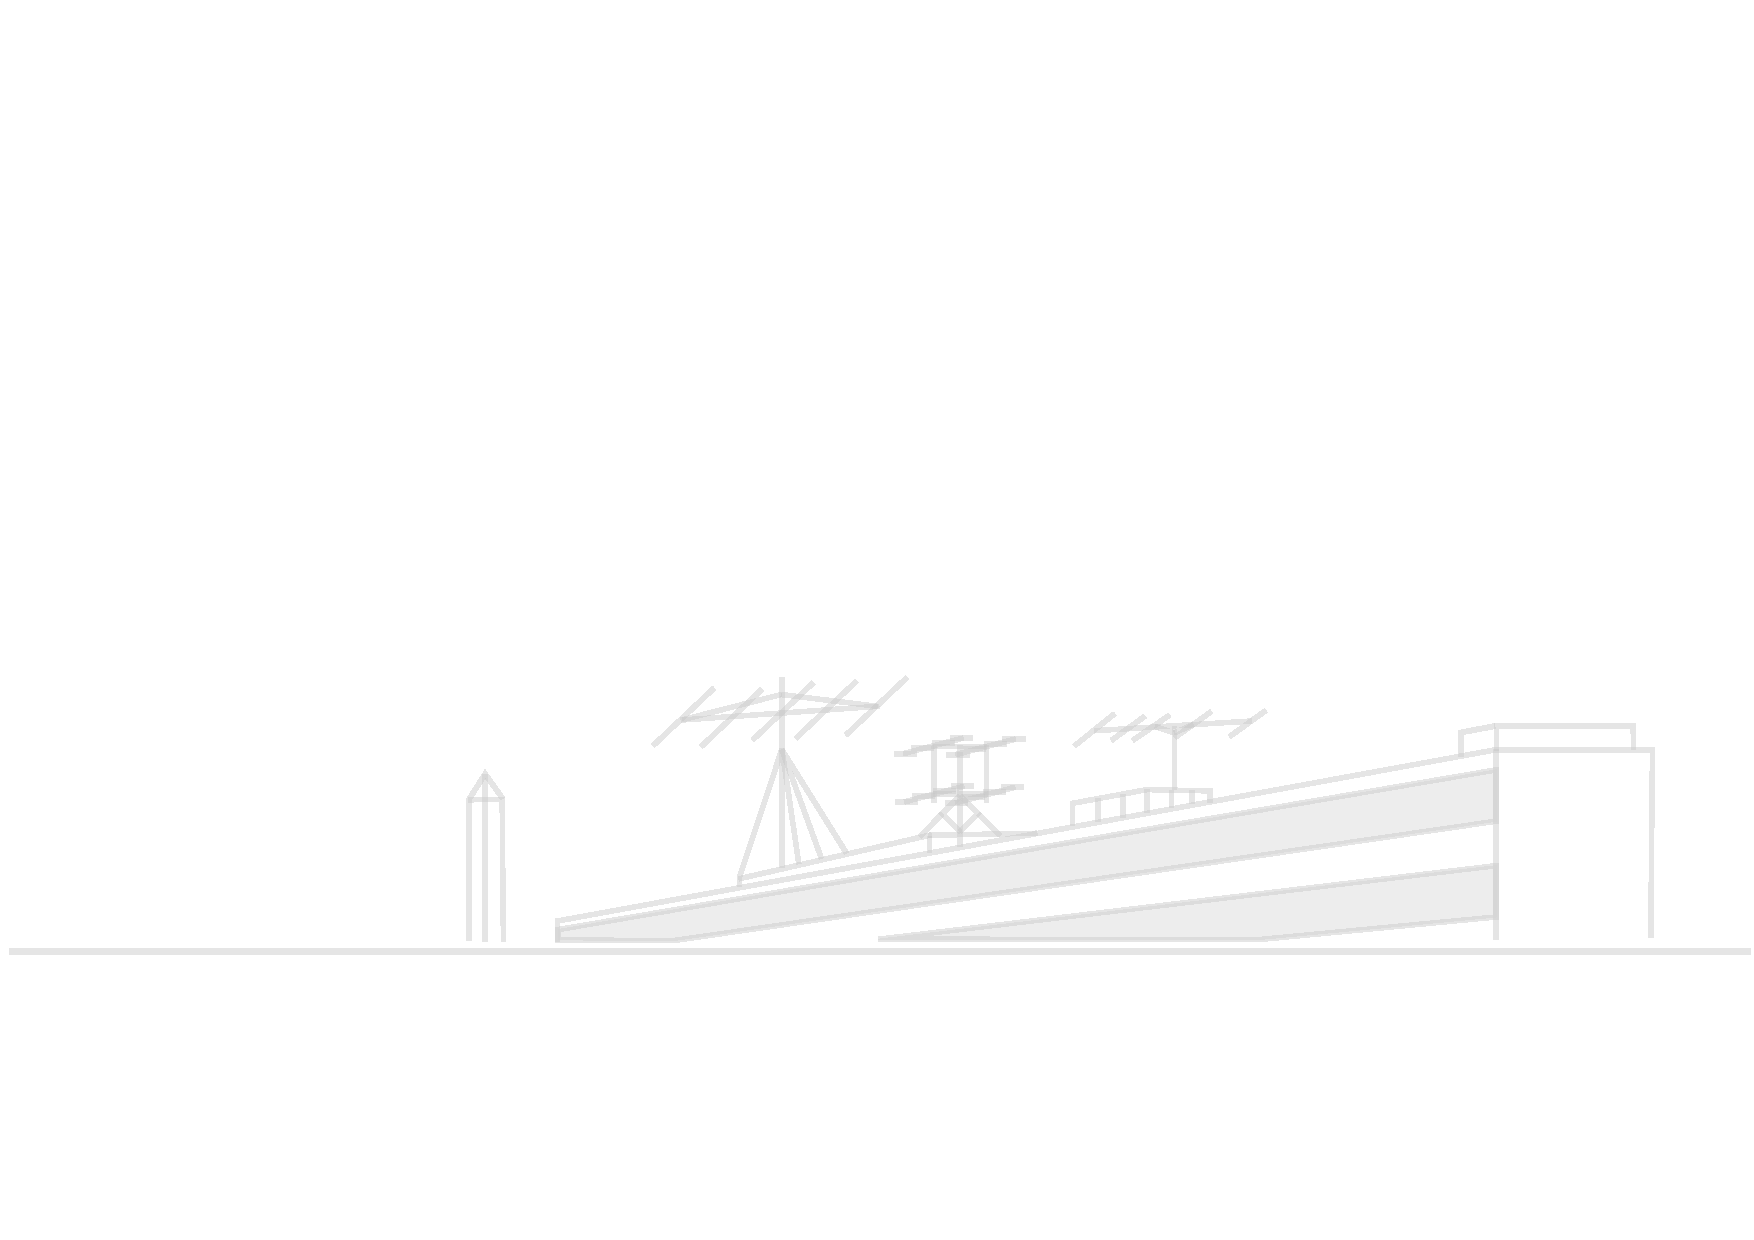
\includegraphics[width=17.8cm]{texdata/dk0tu_rooftop_background.pdf}
}

% Foliennummer einfügen
\setbeamertemplate{footline}[frame number]
%\setbeamertemplate{footline}{}

% Ändere das Zeichen vor jedem item
%\setbeamertemplate{itemize item}{\color{craneorange}$\blacktriangleright$}
%\setbeamertemplate{itemize subitem}{\color{craneorange}$\triangleright$}
%\setbeamertemplate{itemize subsubitem}{\color{craneorange}$\blacktriangleright$}

% Ändert die Blöcke 
\setbeamertemplate{blocks}[rounded][shadow=true]
% default | rounded [shadow=true|false]

%
% Eigene Kommandos
%

% Hack to get natbib and beamer working together. "The beamer user guide suggests
% that only the manual bibliography entry approach is supported"
% on some system it works out of the box, sometimes you need the hack :-(
% so check it --dl7bst
\ifdefined\newblock
    \relax
\else
    \newcommand{\newblock}{}
\fi

% \includedia command to generate png out of a dia file
% NEEDS installed dia and pdflatex option --shell-escape
\newcommand{\includedia}[1]{
    \immediate\write18{/usr/bin/dia #1.dia -e #1_diatmp.png -t png}
}

% RICHIG GROSSER FONT!
\newfont{\bigfont}{cmr10 at 144pt}
\newfont{\smallfont}{cmr10 at 8pt}

% Römische Ziffern
\makeatletter
\newcommand{\rmnum}[1]{\romannumeral #1}
\newcommand{\Rmnum}[1]{\expandafter\@slowromancap\romannumeral #1@}
\makeatother

% Schwarze Überschrift
%\setbeamercolor{frametitle}{fg=black}
%\setbeamercolor{title}{fg=black}

% Item- und Box-Farben
\definecolor{deepBlue}{HTML}{000066}
\setbeamercolor{itemize item}{fg=deepBlue}
\setbeamercolor{itemize subitem}{fg=deepBlue}
\setbeamercolor{description item}{fg=deepBlue}
\setbeamercolor{block title}{fg=deepBlue!100, bg=blue!15}
\setbeamercolor{block body}{fg=black, bg=blue!5}
\setbeamercolor{block title alerted}{fg=deepBlue, bg=red!75}
\setbeamercolor{block body alerted}{fg=black, bg=red!15}
\setbeamercolor*{block title example}{fg=blue!50, bg=blue!10}
\setbeamercolor*{block body example}{fg= blue, bg=blue!5}

%\setbeamercolor{section in head/foot}{parent=palette primary}
%\setbeamercolor{subsection in head/foot}{parent=palette secondary}
%\setbeamercolor{sidebar}{fg=darkblue,bg=yellow!90!orange}
%\setbeamercolor{title in sidebar}{fg=darkblue}
%\setbeamercolor{author in sidebar}{fg=darkblue}
%\setbeamercolor{section in sidebar}{fg=darkblue!10!black}
%\setbeamercolor{subsection in sidebar}{fg=darkblue!50!black}

% Titlepage Infos
\title{AFu-Kurs nach DJ4UF}
\author[DKØTU]{DKØTU\\ \footnotesize{Amateurfunkgruppe der TU Berlin}}
\institute[DKØTU]{\url{http://www.dk0tu.de} }

% PDF-Eigenschaften
\subject{DK0TU-Amateurfunkkurs nach DJ4UF}
\keywords{Amateurfunk Kurs HAM Radio Course CC-BY-NC-SA OpenSource TU Berlin DK0TU}

\subtitle{Betriebstechnik/Vorschriften 01: \\
          Welche Rechte/Pflichten hat ein Funkamateur? \\[2em]}
\date{Stand 22.10.2015}
 \begin{document}

\begin{frame}
    \titlepage
    \vfill
    \begin{center}
        \ccbyncsaeu\\
        {\tiny This work is licensed under the \em{Creative Commons Attribution-NonCommercial-ShareAlike 3.0 License}.}\\[0.5ex]
         \tiny Amateurfunkgruppe der Technische Universität Berlin (AfuTUB), DKØTU
         %\includegraphics[scale=0.5]{img/DK0TU_Logo.pdf}
    \end{center}
\end{frame}


\section{Einleitung}

\subsection{Amateurfunk damals}

\begin{frame}
    \frametitle{Geschichte / HAM -- ein saftiger Schinken?}

    \begin{center}
        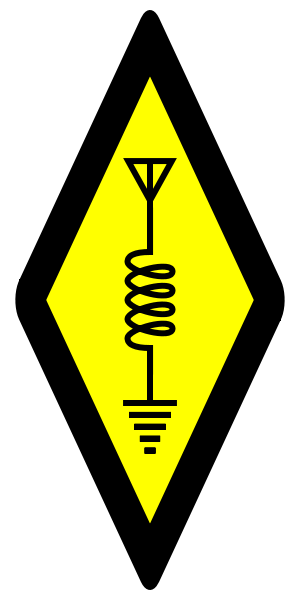
\includegraphics[height=0.3\textheight]{bv01/International_amateur_radio_symbol.png}
        \tiny \hyperlink{refs}{\cite{wc}}
    \end{center}

    \begin{itemize}
        \item Begriff wird für Funkamateure bereits in Pionierzeiten seit Beginn
              des 20.~Jahrhunders verwendet
        \item Bänder und Rufzeichen damals noch völlig unreglementiert
        \item alles andere unbestätigte Mythen
        \begin{itemize}
            \item z.B. bekannteste Legende der drei Amateure \textbf{H}yman,
                  \textbf{A}lmay und \textbf{M}urray
            \item es gibt verschiedene Quellen\hyperlink{refs}{\cite{ham}},
                  die das mal genauer recherchiert haben
        \end{itemize}
    \end{itemize}

\end{frame}

\begin{frame}
    \frametitle{Geschichte / Manifestierung}

    Fakt ist:

    \begin{itemize}
        \item von Beginn an Interessenkonflikte zwischen kommerziellen Stationen
              und Amateuren
        \item Gewerbe wollte zuerst vorrangig Langwelle
        \item \textbf{HAM}s erforschten alles drüber und erweckten neue
              Begehrlichkeiten
        \item durch stetige Arbeit der Amateurfunkverbände gab es dann in
              vielen Bändern ``Häppchen'' für die Hobbyfunker
    \end{itemize}

\end{frame}

\begin{frame}
    \frametitle{Geschichte / Es ist noch nicht vorbei}
 
    \begin{center}
        
\includegraphics[height=0.3\textheight]{bv01/DARC_Logo.pdf}
    \end{center}
   
    \begin{itemize}
        \item Frequenzen heute wertvoller denn je
        \item in Gremien weltweit sitzt ``unsere Lobby''
        \item uns eint kein kommerzielles Interesse, sondern der
              \emph{HAM Spirit}\hyperlink{refs}{\cite{wp}}
    \end{itemize}

\end{frame}

\subsection{Amateurfunk heute}

\begin{frame}
    \frametitle{Amateurfunk -- längst überholtes Hobby?}

    Natürlich ist es kein Problem oder Kostenfaktor mehr mit Leuten auf
    anderen Kontinenten zu kommunizieren. Aber:

    \begin{itemize}
        \item Technik in all ihren Facetten experimentieren
        \item weltweit Gleichgesinnte kennenlernen
        \item egal ob neue Innovation oder gesellschiaftliche Bedeutung -- es beginnt
              immer mit dem Verstehen der technischen Grundlagen
        \item globale autarke P2P-Verbindungen kann eben \textbf{nicht} jeder
        \item direkte Kommunikation ohne Provider weltweit und darüber heraus
        \item ...
    \end{itemize}

\end{frame}

\section{AFu-Zeugnis}

\begin{frame}
    \frametitle{Das Amateurfunkzeugnis}

    Novice Licence (Klasse E)
    
    \begin{itemize}
        \item einfacherer Technikprüfungsteil
        \item erlaubte Bänder und Leistungen eingeschränkt
    \end{itemize}

    Advanced Licence (Klasse A)
    
    \begin{itemize}
        \item Technikfragenkatalog umfangreicher und anspruchsvoller
        \item alle Bänder und Leistungsgrenzen im gesetzlichen Umfang
        \pause
        \item ``die Lizenz zum Löten''
    \end{itemize}

\end{frame}

\subsection{Prüfung}

\begin{frame}
    \frametitle{AFu-Zeugnis / Prüfung}

    schriftliche Prüfung bei der Bundesnetzagentur (BNetzA) mit öffentlichen
    Fragenkatalogen der Bestandteile:

    \begin{itemize}
        \item Technik Klasse E oder A\footnote{bei Upgrade auf Klasse A wird nur
              der Technik-Teil geprüft}
        \item Betriebstechnik
        \item Vorschriften
    \end{itemize}

    \vspace{2em}

    Morseprüfung freiwillig und in DL \textbf{nicht} für das AFu-Zeugnis benötigt

\end{frame}

\begin{frame}
    \frametitle{AFu-Zeugnis / Prüfung}

    Bedingungen:

    \begin{itemize}
        \item \textbf{keine} Beschränkung des Alters oder der Staatsangehörigkeit
        \item Wohnsitz muss in DL sein
    \end{itemize}

    Mit bestandener Prüfung\footnote{mehr Infos: \scriptsize
    \url{http://www.dk0tu.de/Kurse/AFu-Lizenz/FAQ\#prfung}} kann die
    Amateurfunkzulassung beantragt werden.

\end{frame}

\section{AFu-Zulassung}

\begin{frame}
    \frametitle{Die Amateurfunkzulassung}

    Mit der Amateurfunkzulassung wird ein \textbf{personengebundenes(!)}
    Rufzeichen zugewiesen:

    \begin{itemize}
        \item erst ab Zuteilung darf Amateurfunkbetrieb ausgeübt werden
        \item kein Anspruch auf bestimmtes Call
        \item Rufzeichen werden ein Jahr gesperrt\footnote{z.B. bei
              vorübergehender Abmeldung oder nach Tod}
        \item Änderungen der Anschrift der ortsfesten Amateurfunkstelle
              unverzüglich anzeigen
    \end{itemize}

\end{frame}

\section{Rechtliche Eingrenzung}

\subsection{``Funkamateur''}

\begin{frame}
    \frametitle{``Funkamateur''}

    Begriff \emph{Funkamateur} im Sinne des Gesetzes:

    \begin{itemize}
        \item persönliche Neigung
        \item keine gewerblich-wirtschaftlichen Interessen
        \item darf selbst gefertigte oder umgebaute Sendeanlagen auf Amateurfunkfrequenzen betreiben
    \end{itemize}

\end{frame}

\subsection{Verbote}

\begin{frame}
    \frametitle{Verbote}

    nicht erlaubt ist

    \begin{itemize}
        \item Senden ohne Zulassung (Rufzeichen)
        \item gewerblich-wirtschaftliche Zwecke
        \item Übermitteln von Nachrichten an Dritte
        \item Nutzung von Frequenzen außerhalb des zugelassenen Nutzungsbereichs
        \item Funkverkehr mit Nicht-Amateurfunkstellen\footnote{außer in Notfällen}
        \item Übermittlung von verschlüsselten Nachrichten zum Zwecke der Verschleierung
        \item religiöse oder politische Inhalte
        \item rundfunkähnliche Aussendungen
    \end{itemize}

\end{frame}

\subsection{Strafen}

\begin{frame}
    \frametitle{Strafen}

    Die Bundesnetzagentur kann anordnen:

    \begin{itemize}
        \item Einschränkung des Betriebs oder Außerbetriebnahme der
              Amateurfunkstelle\footnote{Betrieb einer Amateurfunkstelle ohne
              AFu-Zulassung ist eine Ordnungswidrigkeit}
        \item Geldbuße
        \begin{itemize}
            \item bei Nichtzahlung ggf. Maßnahmen nach Verwaltungs-Vollstreckungsgesetz
        \end{itemize}
        \item Entzug der \emph{Zulassung zur Teilnahme am Amateurfunkdienst}
    \end{itemize}

    \vspace{1em}

    Beachte: Amateurfunkzeugnis und Sendeanlage\footnote{wenn keine Straftat
    damit verübt wurde} können nicht entzogen werden

\end{frame}

\begin{frame}

    \begin{alertblock}{Hausaufgabe (fakultativ)}
        Amateurfunkgesetz (AFuG, 13 Paragraphen auf 4 DIN-A4-Seiten) und
        Amateurfunkverordnung (AfuV, 20 Paragraphen + Anlagen auf 11
        DIN-A4-Seiten) einmal querlesen.
    \end{alertblock}

\end{frame}

\renewcommand{\refname}{Referenzen}

\begin{frame}
    \frametitle{Referenzen/Links}
    \hypertarget{refs}{}
    \footnotesize

    \begin{thebibliography}{}
        \bibitem{dj4uf} Moltrecht B/V 01: \\
                        \url{http://www.amateurfunkpruefung.de/lehrg/bv01/bv01.html}
        \bibitem{wp}    Wikipedia DE: \\
                        \url{http://de.wikipedia.org/wiki/Ham_Spirit} \\
        \bibitem{ham}   Recherchen zum Begriff ''HAM'':
                        \url{http://www.indyradioclub.org/wordham.pdf} \\
                        \url{http://www.w7eca.org/FILES/y_ham.doc} \\
                        \url{http://www.hotarc.org/files/origin_of_HAM_by_KN4AQ.pdf}
        \bibitem{wc}    Wikimedia Commons: \\
                        \url{http://commons.wikimedia.org/wiki/File:International_amateur_radio_symbol.svg}
    \end{thebibliography} 
   
\end{frame}

% Hier könnte noch eine Kontaktfolie stehen

\end{document}

